\documentclass[11pt,a4paper,fontset=none]{ctexart}
\usepackage{fontspec}
\usepackage{xeCJK}
\usepackage{amsmath,amssymb,mathtools}
\usepackage{geometry}
\usepackage[dvipsnames]{xcolor}
\usepackage{tikz}
\usetikzlibrary{
  arrows.meta,
  angles,
  backgrounds,
  calc,
  decorations.markings,
  decorations.pathmorphing,
  decorations.pathreplacing,
  fit,
  intersections,
  matrix,
  patterns,
  patterns.meta,
  positioning,
  quotes,
  shapes.geometric,
  shapes.misc,
  through,
  3d
}
\usepackage{pgfplots}
\pgfplotsset{compat=1.18}
\usepackage[most]{tcolorbox}
\usepackage{enumitem}
\usepackage{multicol}
\usepackage{tabularx,array,booktabs,multirow}
\usepackage{fancyhdr}
\usepackage{lastpage}
\usepackage{titlesec}
\usepackage{needspace}
\usepackage{eso-pic}
\usepackage{graphicx}
\usepackage{hyperref}
\usepackage{xparse}

\geometry{
  a4paper,
  left=18mm,
  right=18mm,
  top=22mm,
  bottom=20mm,
  headheight=22pt,
  headsep=8mm,
  footskip=11mm
}

\setmainfont{texgyrepagella-regular.otf}[
  BoldFont=texgyrepagella-bold.otf,
  ItalicFont=texgyrepagella-italic.otf,
  BoldItalicFont=texgyrepagella-bolditalic.otf
]
\setsansfont{texgyreheros-regular.otf}[
  BoldFont=texgyreheros-bold.otf,
  ItalicFont=texgyreheros-italic.otf,
  BoldItalicFont=texgyreheros-bolditalic.otf
]
\setmonofont{texgyrecursor-regular.otf}[
  BoldFont=texgyrecursor-bold.otf
]
\setCJKmainfont{Kaiti SC}[
  BoldFont=Kaiti SC
]
\setCJKsansfont{FandolHei-Regular.otf}[
  BoldFont=FandolHei-Bold.otf
]
\setCJKmonofont{FandolKai-Regular.otf}

\definecolor{Paper}{HTML}{FBFCFA}
\definecolor{Ink}{HTML}{17324D}
\definecolor{Muted}{HTML}{647784}
\definecolor{Teal}{HTML}{167D89}
\definecolor{TealDark}{HTML}{0F5F69}
\definecolor{Mint}{HTML}{E8F5F2}
\definecolor{Sky}{HTML}{EAF3F8}
\definecolor{Coral}{HTML}{E66A5A}
\definecolor{Gold}{HTML}{D7A94A}
\definecolor{Rule}{HTML}{C8D8DA}
\definecolor{SolutionBg}{HTML}{FFF9F1}

\pagecolor{Paper}
\color{Ink}
\linespread{1.14}
\setlength{\parindent}{2em}
\setlength{\parskip}{0.25em}
\setlength{\columnsep}{1.3cm}
\setlength{\abovedisplayskip}{0.7em}
\setlength{\belowdisplayskip}{0.7em}
\setlist{nosep}

\hypersetup{
  colorlinks=true,
  linkcolor=TealDark,
  urlcolor=TealDark,
  pdfborder={0 0 0}
}

\newcommand{\papertitle}{Mathstalents 小学版练习题}
\newcommand{\SetPaperTitle}[1]{\renewcommand{\papertitle}{#1}}

\pagestyle{fancy}
\fancyhf{}
\fancyhead[L]{\sffamily\small\color{TealDark}\papertitle}
\fancyhead[R]{}
\fancyfoot[C]{%
  {\sffamily\scriptsize\color{Muted}第~\arabic{page}~页~/~共~\pageref*{LastPage}~页}%
}
\renewcommand{\headrulewidth}{0.4pt}
\renewcommand{\footrulewidth}{0pt}
\renewcommand{\headrule}{\hbox to\headwidth{\color{Rule}\leaders\hrule height \headrulewidth\hfill}}

\AddToShipoutPictureBG{%
  \begin{tikzpicture}[remember picture,overlay]
    \draw[Rule,line width=0.35pt,rounded corners=2pt]
      ([xshift=6mm,yshift=-6mm]current page.north west)
      rectangle
      ([xshift=-6mm,yshift=6mm]current page.south east);
    \draw[Teal,line width=1.1pt]
      ([xshift=6mm,yshift=-14mm]current page.north west) --
      ([xshift=6mm,yshift=-6mm]current page.north west) --
      ([xshift=14mm,yshift=-6mm]current page.north west);
    \draw[Coral,line width=1.1pt]
      ([xshift=-6mm,yshift=14mm]current page.south east) --
      ([xshift=-6mm,yshift=6mm]current page.south east) --
      ([xshift=-14mm,yshift=6mm]current page.south east);
  \end{tikzpicture}%
}

\newcommand{\metachip}[2][Teal]{%
  \tikz[baseline=(chip.base)]\node[
    fill=#1!10,
    draw=#1!45,
    text=#1!80!black,
    rounded corners=2.5pt,
    inner xsep=6pt,
    inner ysep=2.4pt,
    font=\sffamily\scriptsize
  ] (chip) {\textbf{#2}};%
}

\NewDocumentCommand{\makecover}{m m m m m m}{%
  \thispagestyle{empty}
  \begin{tikzpicture}[remember picture,overlay]
    \draw[Teal!14,line width=0.8pt,step=10mm]
      ([xshift=8mm,yshift=8mm]current page.south west) grid
      ([xshift=-8mm,yshift=-8mm]current page.north east);
    \node[
      anchor=north west,
      text=Ink,
      align=left,
      text width=155mm
    ] at ([xshift=24mm,yshift=-35mm]current page.north west) {
      {\sffamily\bfseries\fontsize{14}{18}\selectfont
        MATHSTALENTS \(\cdot\) ELEMENTARY}\\[9mm]
      {\sffamily\bfseries\fontsize{34}{42}\selectfont
        小学版 \(\,\boldsymbol{\cdot}\,\) #1}\\[3mm]
      {\sffamily\fontsize{17}{23}\selectfont
        练习题与参考答案}\\[11mm]
      {\color{TealDark}\rule{112mm}{1.1pt}}\\[7mm]
      {\sffamily\fontsize{13}{20}\selectfont #2}
    };
    \node[
      anchor=north west,
      fill=white,
      draw=TealDark,
      line width=0.6pt,
      text opacity=1,
      rounded corners=5pt,
      inner sep=9mm,
      text width=137mm
    ] at ([xshift=24mm,yshift=-126mm]current page.north west) {
      \begin{minipage}{137mm}
        \sffamily
        \begin{tabularx}{\linewidth}{>{\centering\arraybackslash}X
          >{\centering\arraybackslash}X
          >{\centering\arraybackslash}X}
          {\color{TealDark}\bfseries\Large #3} &
          {\color{TealDark}\bfseries\Large #4} &
          {\color{TealDark}\bfseries\Large 精编}\\[-1mm]
          {\color{Muted}\small 总分} &
          {\color{Muted}\small 题目数} &
          {\color{Muted}\small 题解版本}
        \end{tabularx}
        \vspace{6mm}
        {\color{Rule}\hrule}
        \vspace{5mm}
        {\color{Ink}\bfseries 题型结构}\par
        \vspace{2mm}
        {\color{Muted}\small #5}
      \end{minipage}
    };
  \end{tikzpicture}
  \null
  \clearpage
}

\newcommand{\paperinfo}[3]{%
  \begin{tcolorbox}[
    enhanced,
    colback=Sky,
    colframe=Teal!40,
    boxrule=0.6pt,
    arc=3pt,
    left=5mm,right=5mm,top=4mm,bottom=4mm
  ]
    \sffamily
    \begin{tabularx}{\linewidth}{@{}X X X@{}}
      \textbf{姓名：}\rule{28mm}{0.4pt} &
      \textbf{用时：}\rule{22mm}{0.4pt} &
      \textbf{得分：}\rule{22mm}{0.4pt}\\[3mm]
      \multicolumn{3}{@{}l@{}}{\small\color{Muted}
        #1 \qquad #2 \qquad #3}
    \end{tabularx}
  \end{tcolorbox}
  \vspace{2mm}
}

\newcommand{\mtQuestionNeedspace}{8.2cm}
\newcommand{\mtBannerNeedspace}{6.8cm}
\newcommand{\mtQuestionBreakLines}{8}

\newcommand{\sectionbanner}[2]{%
  \Needspace{\mtBannerNeedspace}
  \begin{tcolorbox}[
    enhanced,
    colback=white,
    colframe=TealDark,
    boxrule=0.65pt,
    arc=2.5pt,
    left=4mm,right=4mm,top=2.6mm,bottom=2.6mm,
    before skip=3.2mm,
    after skip=2.2mm
  ]
    {\sffamily\bfseries\large\color{TealDark}#1\quad
     \sffamily\small #2}
  \end{tcolorbox}
}

\NewDocumentEnvironment{question}{m m}{%
  \Needspace{\mtQuestionNeedspace}
  \begin{tcolorbox}[
    enhanced,
    breakable,
    lines before break=\mtQuestionBreakLines,
    colback=white,
    colframe=Rule,
    boxrule=0.55pt,
    arc=3pt,
    left=5mm,right=5mm,top=5mm,bottom=4mm,
    before skip=4mm,
    after skip=4mm,
    title={\sffamily\bfseries 第 #1 题（ #2 分 ）},
    coltitle=TealDark,
    colbacktitle=white,
    fonttitle=\sffamily\bfseries,
    attach boxed title to top left={xshift=4mm,yshift=-2.8mm},
    boxed title style={
      colback=white,
      colframe=TealDark,
      arc=2.5pt,
      boxrule=0.65pt,
      left=3mm,right=3mm,top=1.5mm,bottom=1.5mm
    }
  ]
  \hypertarget{question:#1}{}%
  \vspace{1mm}
}{%
  \end{tcolorbox}
}

\ExplSyntaxOn
\seq_new:N \g_mt_choices_seq
\dim_new:N \l_mt_choice_max_dim
\dim_new:N \l_mt_choice_sum_dim
\dim_new:N \l_mt_choice_tmp_dim
\dim_new:N \l_mt_choice_label_dim
\box_new:N \l_mt_choice_box

\NewDocumentCommand{\choice}{m}
{
  \seq_gput_right:Nn \g_mt_choices_seq {#1}
}

\cs_new_protected:Npn \mt_set_choice_label_dim:
{
  \hbox_set:Nn \l_mt_choice_box
  {
    \textcolor{TealDark}{\bfseries E.}
    \hspace{0.45em}
  }
  \dim_set:Nn \l_mt_choice_label_dim { \box_wd:N \l_mt_choice_box }
}

\cs_new_protected:Npn \mt_choice_label:n #1
{
  \textcolor{TealDark}{\bfseries \int_to_Alph:n {#1}.}
}

\cs_new_protected:Npn \mt_typeset_choice:nn #1#2
{
  \mt_choice_label:n {#1}\hspace{0.45em}#2
}

\cs_new_protected:Npn \mt_typeset_choice_par:nn #1#2
{
  \par\noindent
  \hangindent = \l_mt_choice_label_dim
  \hangafter = 1
  \makebox[\l_mt_choice_label_dim][l]{ \mt_choice_label:n {#1} }
  #2
  \par
}

\cs_new_protected:Npn \mt_measure_choices:
{
  \dim_zero:N \l_mt_choice_max_dim
  \dim_zero:N \l_mt_choice_sum_dim
  \int_step_inline:nn { \seq_count:N \g_mt_choices_seq }
  {
    \hbox_set:Nn \l_mt_choice_box
    {
      \mt_typeset_choice:nn {##1} { \seq_item:Nn \g_mt_choices_seq {##1} }
    }
    \dim_set:Nn \l_mt_choice_tmp_dim { \box_wd:N \l_mt_choice_box }
    \dim_set:Nn \l_mt_choice_sum_dim { \l_mt_choice_sum_dim + \l_mt_choice_tmp_dim + 1.6em }
    \dim_set:Nn \l_mt_choice_max_dim
    {
      \dim_max:nn { \l_mt_choice_max_dim } { \l_mt_choice_tmp_dim }
    }
  }
}

\cs_new_protected:Npn \mt_print_choices:
{
  \mt_set_choice_label_dim:
  \mt_measure_choices:
  \par\nopagebreak\vspace{0.5em}
  \dim_compare:nNnTF { \l_mt_choice_sum_dim } < { \linewidth }
  {
    \noindent
    \int_step_inline:nn { \seq_count:N \g_mt_choices_seq }
    {
      \mbox
      {
        \mt_typeset_choice:nn {##1} { \seq_item:Nn \g_mt_choices_seq {##1} }
      }
      \hfill
    }
    \par
  }
  {
    \dim_compare:nNnTF { \l_mt_choice_max_dim + 0.6em } < { 0.5\linewidth }
    {
      \noindent
      \int_step_inline:nn { \seq_count:N \g_mt_choices_seq }
      {
        \begin{minipage}[t]{0.48\linewidth}
          \raggedright
          \mt_typeset_choice_par:nn {##1} { \seq_item:Nn \g_mt_choices_seq {##1} }
        \end{minipage}
        \int_if_odd:nTF {##1}
        { \hfill }
        { \par\vspace{0.38em} }
      }
      \int_if_odd:nT { \seq_count:N \g_mt_choices_seq } { \par }
    }
    {
      \int_step_inline:nn { \seq_count:N \g_mt_choices_seq }
      {
        \mt_typeset_choice_par:nn {##1} { \seq_item:Nn \g_mt_choices_seq {##1} }
        \vspace{0.28em}
      }
    }
  }
  \vspace{0.25em}
  \seq_gclear:N \g_mt_choices_seq
}

\NewDocumentEnvironment{choices}{}
{
  \seq_gclear:N \g_mt_choices_seq
}
{
  \mt_print_choices:
}

\NewDocumentEnvironment{multichoices}{}
{
  \seq_gclear:N \g_mt_choices_seq
}
{
  \mt_print_choices:
}
\ExplSyntaxOff

\NewDocumentCommand{\subquestion}{m m}{%
  \par\medskip
  \noindent
  \metachip[Coral]{#1 分}\hspace{0.7em}#2\par
}

\newcommand{\answerlineskip}{9mm}

\newcommand{\answerspace}{%
  \par\vspace{12mm}%
}

\newcommand{\answerline}{%
  \ifmmode
    \underline{\hspace{2.8cm}}%
  \else
    \ifvmode
      \par\vspace{\answerlineskip}%
      \noindent{\color{Ink}\rule{0.46\linewidth}{0.5pt}}%
      \par\vspace{2.5mm}%
    \else
      \underline{\hspace{2.8cm}}%
    \fi
  \fi
}

\NewDocumentCommand{\answerbox}{m}{%
  \par\vspace{3mm}
  \begin{tcolorbox}[
    enhanced,
    colback=white,
    colframe=Teal!38!Rule,
    boxrule=0.7pt,
    arc=2.5pt,
    left=3.5mm,
    right=3.5mm,
    top=3mm,
    bottom=3mm,
    height=#1,
    before skip=0pt,
    after skip=2mm
  ]
    \mbox{}
  \end{tcolorbox}
}

\NewDocumentEnvironment{solution}{m m m m}{%
  \Needspace{5.4cm}
  \begin{tcolorbox}[
    enhanced,
    breakable,
    lines before break=6,
    colback=white,
    colframe=Gold!65!Ink,
    boxrule=0.6pt,
    arc=3pt,
    left=5mm,right=5mm,top=5mm,bottom=4mm,
    before skip=4mm,
    after skip=4mm,
    title={\sffamily\bfseries 第 #1 题 \(\cdot\) 参考解答},
    coltitle=Ink,
    colbacktitle=white,
    fonttitle=\sffamily\bfseries,
    attach boxed title to top left={xshift=4mm,yshift=-2.8mm},
    boxed title style={
      colback=white,
      colframe=Gold!65!Ink,
      arc=2.5pt,
      boxrule=0.65pt,
      left=3mm,right=3mm,top=1.5mm,bottom=1.5mm
    }
  ]
  \hypertarget{solution:#1}{}%
  \vspace{1mm}
  \noindent
  \metachip[Coral]{答案：#2}\hspace{0.45em}
  \metachip[Gold]{难度：#3}\hspace{0.45em}
  \metachip[Teal]{#4}
  \par\medskip
}{%
  \end{tcolorbox}
}

\NewDocumentCommand{\analysis}{+m}{%
  \par\smallskip
  {\sffamily\bfseries\color{TealDark}思路分析}\par
  \vspace{1mm}
  #1
  \par\smallskip
}

\NewDocumentCommand{\methodsummary}{+m}{%
  \par\medskip
  \noindent
  {\sffamily\bfseries\color{TealDark}方法总结}\quad
  {\sffamily\color{Ink}#1}\par
}

\newcommand{\solutiondivider}{%
  \clearpage
}

\renewcommand{\mtQuestionNeedspace}{3.2cm}
\renewcommand{\mtBannerNeedspace}{2.0cm}
\renewcommand{\mtQuestionBreakLines}{3}

\SetPaperTitle{Mathstalents 小学版 · 第三套卷}
\hypersetup{
  pdftitle={Mathstalents 小学版第三套卷：练习题与参考答案},
  pdfauthor={重新录入与排版}
}

\begin{document}
\raggedbottom

\makecover
  {第三套卷}
  {2026 年 7 月 18 日}
  {150}
  {22}
  {单选题 \(10\times5\) 分 \(\cdot\)
   多选题 \(4\times7\) 分 \(\cdot\)
   填空题 \(5\times6\) 分 \(\cdot\)
   综合题 \(3\times14\) 分}
  {第三套卷 \(\cdot\) 题目、参考答案与矢量重绘图}

\paperinfo{满分 150 分}{共 22 题}{建议用时 120 分钟}
% UTF-8 LaTeX fragment: questions only

\sectionbanner{一、单选题}{共10题，每题5分，共50分}

\begin{question}{1}{5}
数列满足 \(a_1=1,\ a_2=3\)，且从第3项开始，每后一项都等于前两项之和。前30项中有多少项是偶数？
\begin{choices}
  \choice{8}
  \choice{9}
  \choice{10}
  \choice{11}
\end{choices}
\end{question}

\begin{question}{2}{5}
三盏灯从同一时刻开始同时亮起，此后红灯每6分钟亮一次，蓝灯每10分钟亮一次，绿灯每15分钟亮一次。在开始后的3小时内，不含开始时刻，三盏灯同时亮起多少次？
\begin{choices}
  \choice{4}
  \choice{5}
  \choice{6}
  \choice{7}
\end{choices}
\end{question}

\begin{question}{3}{5}
正整数 \(a,b\) 满足 \(a+b=60\)，且 \(a\) 与 \(b\) 的最大公因数为12。\(ab\) 的最大值是多少？
\begin{choices}
  \choice{720}
  \choice{864}
  \choice{1008}
  \choice{1152}
\end{choices}
\end{question}

\begin{question}{4}{5}
已知图1（Figure 1）显示了一个直径为 \(9\text{ cm}\) 的圆。图2（Figure 2）显示了一个由五个圆组成的奥运标志，每个圆的直径都是 \(9\text{ cm}\)。如图所示，下层左圆的最左端与上层左圆的最右端之间的水平距离为 \(4\text{ cm}\)。请问该奥运标志（Figure 3）的总长度是多少厘米？

% Source figure: assets/original/page-04.png
\begin{center}
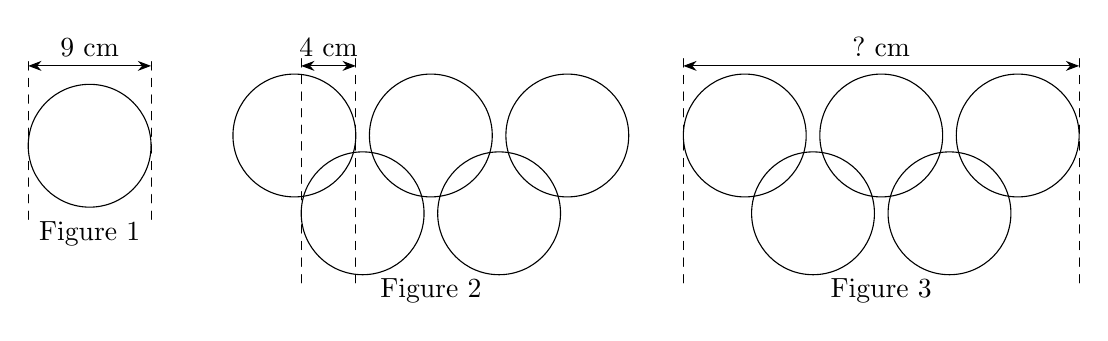
\begin{tikzpicture}[x=0.52cm,y=0.52cm,>=Stealth,line cap=round,line join=round]
  % Figure 1
  \begin{scope}
    \draw (0,0) circle (1.5);
    \draw[dashed] (-1.5,-1.8)--(-1.5,2.1);
    \draw[dashed] (1.5,-1.8)--(1.5,2.1);
    \draw[<->] (-1.5,1.95)--node[above] {\(9\text{ cm}\)} (1.5,1.95);
    \node at (0,-2.15) {Figure 1};
  \end{scope}

  % Figure 2
  \begin{scope}
    \foreach \x in {5,8.333,11.666} {
      \draw (\x,0.25) circle (1.5);
    }
    \foreach \x in {6.667,10} {
      \draw (\x,-1.65) circle (1.5);
    }
    \draw[dashed] (5.167,-3.35)--(5.167,2.15);
    \draw[dashed] (6.5,-3.35)--(6.5,2.15);
    \draw[<->] (5.167,1.95)--node[above] {\(4\text{ cm}\)} (6.5,1.95);
    \node at (8.333,-3.55) {Figure 2};
  \end{scope}

  % Figure 3
  \begin{scope}
    \foreach \x in {16,19.333,22.666} {
      \draw (\x,0.25) circle (1.5);
    }
    \foreach \x in {17.667,21} {
      \draw (\x,-1.65) circle (1.5);
    }
    \draw[dashed] (14.5,-3.35)--(14.5,2.15);
    \draw[dashed] (24.166,-3.35)--(24.166,2.15);
    \draw[<->] (14.5,1.95)--node[above] {\(?\text{ cm}\)} (24.166,1.95);
    \node at (19.333,-3.55) {Figure 3};
  \end{scope}
\end{tikzpicture}
\end{center}

\begin{choices}
  \choice{\(25\text{ cm}\)}
  \choice{\(27\text{ cm}\)}
  \choice{\(28\text{ cm}\)}
  \choice{\(29\text{ cm}\)}
  \choice{\(30\text{ cm}\)}
\end{choices}
\end{question}

\begin{question}{5}{5}
同时掷两枚普通骰子，已知两枚骰子的点数乘积能被4整除。在这个条件下，两枚骰子的点数和为偶数的概率是多少？
\begin{choices}
  \choice{\(\dfrac25\)}
  \choice{\(\dfrac7{15}\)}
  \choice{\(\dfrac35\)}
  \choice{\(\dfrac23\)}
\end{choices}
\end{question}

\begin{question}{6}{5}
请问图中一共有多少个三角形？

% Source figure: assets/original/page-06.png
{\centering
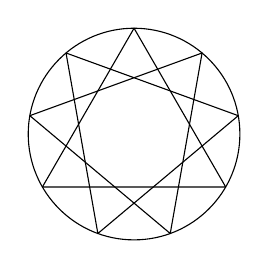
\begin{tikzpicture}[scale=0.56,line cap=round,line join=round]
  \draw (0,0) circle (2.4);
  \foreach \r in {-40,0,40} {
    \draw ({90+\r}:2.4)--({210+\r}:2.4)--({330+\r}:2.4)--cycle;
  }
\end{tikzpicture}\par}

\begin{choices}
  \choice{27}
  \choice{30}
  \choice{25}
  \choice{32}
  \choice{35}
\end{choices}
\end{question}

\begin{question}{7}{5}
数列满足 \(a_1=5\)，且从第1项开始，每后一项都等于前一项的2倍再加1。\(a_{20}+a_{21}\) 除以7的余数是多少？
\begin{choices}
  \choice{3}
  \choice{4}
  \choice{5}
  \choice{6}
\end{choices}
\end{question}

\begin{question}{8}{5}
当哲哲在下午5:00之后不久开始慢跑时，他注意到他的指针式手表的时针和分针形成了一个 \(99^\circ\) 的夹角。当他在下午6:00之前结束慢跑时，他发现两根指针再次形成了一个 \(99^\circ\) 的夹角。请问哲哲慢跑了多少分钟？

% Source figure: assets/original/page-08.png
{\centering
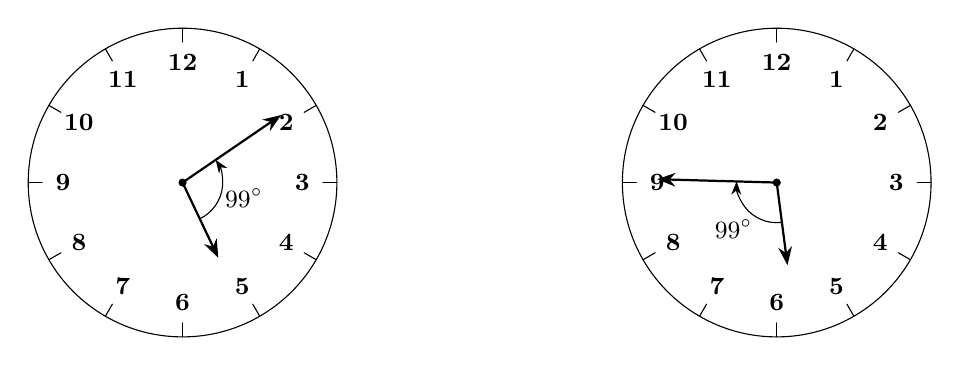
\begin{tikzpicture}[scale=0.98,>=Stealth,line cap=round,line join=round]
  \begin{scope}[xshift=-3.85cm]
    \draw (0,0) circle (2);
    \foreach \a in {0,30,...,330} {
      \draw (\a:1.82)--(\a:2);
    }
    \foreach \n/\a in {12/90,1/60,2/30,3/0,4/-30,5/-60,6/-90,7/-120,8/-150,9/180,10/150,11/120} {
      \node[font=\bfseries\small] at (\a:1.55) {\n};
    }
    \fill (0,0) circle (1.5pt);
    \draw[->,thick] (0,0)--(34.4:1.55);
    \draw[->,thick] (0,0)--(-64.6:1.08);
    \draw[->] (-64.6:0.52) arc[start angle=-64.6,end angle=34.4,radius=0.52];
    \node[font=\small] at (-14:0.82) {\(99^\circ\)};
  \end{scope}
  \begin{scope}[xshift=3.85cm]
    \draw (0,0) circle (2);
    \foreach \a in {0,30,...,330} {
      \draw (\a:1.82)--(\a:2);
    }
    \foreach \n/\a in {12/90,1/60,2/30,3/0,4/-30,5/-60,6/-90,7/-120,8/-150,9/180,10/150,11/120} {
      \node[font=\bfseries\small] at (\a:1.55) {\n};
    }
    \fill (0,0) circle (1.5pt);
    \draw[->,thick] (0,0)--(178.4:1.55);
    \draw[->,thick] (0,0)--(-82.6:1.08);
    \draw[->] (-82.6:0.52) arc[start angle=-82.6,end angle=-181.6,radius=0.52];
    \node[font=\small] at (-133:0.82) {\(99^\circ\)};
  \end{scope}
\end{tikzpicture}\par}

\begin{choices}
  \choice{34}
  \choice{35}
  \choice{36}
  \choice{37}
  \choice{38}
\end{choices}
\end{question}

\begin{question}{9}{5}
正数 \(a,b\) 满足 \(a+b=18\)，且 \(\dfrac{a}{b}+\dfrac{b}{a}=\dfrac{5}{2}\)。\(ab\) 等于多少？
\begin{choices}
  \choice{60}
  \choice{66}
  \choice{72}
  \choice{78}
\end{choices}
\end{question}

\begin{question}{10}{5}
用数字1、2、3、4、5、6中的4个不同数字排成一列，要求前两个数字之和大于后两个数字之和。共有多少种排法？
\begin{choices}
  \choice{144}
  \choice{148}
  \choice{152}
  \choice{156}
\end{choices}
\end{question}

\sectionbanner{多选题}{共4题，每题7分，共28分}

\begin{question}{11}{7}
每套书签12元，每盒彩笔8元。小林两种都买，共花96元。判断下列说法中哪些一定正确。
\begin{multichoices}
  \choice{书签的套数一定是偶数}
  \choice{彩笔的盒数可以是5}
  \choice{两种物品一共可以买10件}
  \choice{书签最多可以买6套}
\end{multichoices}
\end{question}

\begin{question}{12}{7}
设 \(N=2^3\times3^2\times5\)。判断下列说法中哪些一定正确。
\begin{multichoices}
  \choice{\(N\) 有24个正因数}
  \choice{\(N\) 有6个奇正因数}
  \choice{\(N\) 的正因数中，能被15整除的有8个}
  \choice{\(N\) 的正因数中，完全平方数有6个}
\end{multichoices}
\end{question}

\begin{question}{13}{7}
三堆棋子分别有7枚、10枚、13枚。每次操作选择一堆放入2枚棋子，同时从另外两堆各取走1枚棋子。判断下列说法中哪些一定正确。
\begin{multichoices}
  \choice{三堆棋子的总数始终不变}
  \choice{有奇数枚棋子的堆数始终是偶数}
  \choice{可以经过若干次操作后使三堆棋子都为10枚}
  \choice{每一堆棋子数的奇偶性都保持不变}
\end{multichoices}
\end{question}

\begin{question}{14}{7}
正整数 \(a,b\) 满足 \(a+b=18\)。判断下列说法中哪些一定正确。
\begin{multichoices}
  \choice{\(ab\) 的最大值是81}
  \choice{\(a^2+b^2\) 一定是偶数}
  \choice{如果 \(ab\) 能被17整除，那么 \(a,b\) 中有一个数是17}
  \choice{\(ab\) 可以等于70}
\end{multichoices}
\end{question}

\sectionbanner{二、填空题}{共5题，每题6分，共30分}

\begin{question}{15}{6}
从1到12中任取两个不同的数，使它们的和能被3整除。不计顺序，这样的取法有\underline{\hspace{1.35cm}}种。
\end{question}

\begin{question}{16}{6}
在一个 \(3\times6\) 的表格中，有多少对儿单位正方形没有公共点？图中显示了满足条件的其中一对儿。

% Source figure: assets/original/page-16.png
\noindent
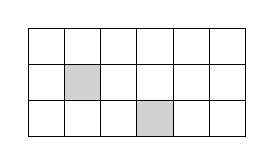
\begin{tikzpicture}[x=0.46cm,y=0.46cm]
  \fill[gray!35] (1,1) rectangle (2,2);
  \fill[gray!35] (3,0) rectangle (4,1);
  \draw[step=1] (0,0) grid (6,3);
\end{tikzpicture}

\end{question}

\begin{question}{17}{6}
黑板上写着1到30这30个整数。每次擦去两个数，再写上这两个数的和。重复操作直到黑板上只剩一个数。最后剩下的数是 \answerline。
\end{question}

\begin{question}{18}{6}
一个正方形被两条线分成了四块。已知其中三块的面积分别是 \(350\text{ m}^2\)、\(163\text{ m}^2\)、\(56\text{ m}^2\)，求最后一块（顶部四边形）的面积是多少平方米？

% Source figure: assets/original/page-18.png
\noindent
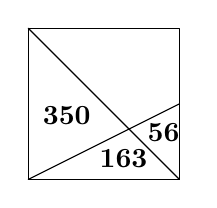
\begin{tikzpicture}[line cap=round,line join=round,scale=0.48]
  \coordinate (P) at (2.86,1.43);
  \draw (0,0) rectangle (4,4);
  \draw (0,4)--(4,0);
  \draw (0,0)--(4,2.00);
  \node[font=\bfseries] at (1.02,1.70) {350};
  \node[font=\bfseries] at (2.52,0.55) {163};
  \node[font=\bfseries] at (3.58,1.25) {56};
\end{tikzpicture}

\end{question}

\enlargethispage{8mm}
\begin{question}{19}{6}
9个互不相同的正整数的平均数为18，其中最小的数是6。这些数中最大数的最小可能值是 \answerline。
\end{question}

\sectionbanner{三、综合题}{共3题，每题14分，共42分}

\begin{question}{20}{14}
标有1到7数字的正六边形灯按右图排列。按下每个灯时，点亮和熄灭的状态会按照以下规则进行切换：

% Source figure: assets/original/page-20.png
{\centering
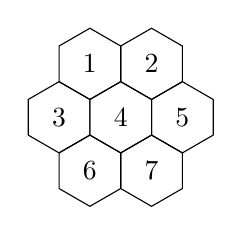
\begin{tikzpicture}[scale=0.78,line cap=round,line join=round]
  \foreach \x/\y/\n in {-0.502/0.87/1,0.502/0.87/2,-1.004/0/3,0/0/4,1.004/0/5,-0.502/-0.87/6,0.502/-0.87/7} {
    \draw ({\x},{\y+0.58})--({\x+0.502},{\y+0.29})--
          ({\x+0.502},{\y-0.29})--({\x},{\y-0.58})--
          ({\x-0.502},{\y-0.29})--({\x-0.502},{\y+0.29})--cycle;
    \node at (\x,\y) {\n};
  }
\end{tikzpicture}\par}

被按下的灯，其点亮/熄灭状态切换。

在与被按下的灯相邻的灯中，只有数字大于被按下的灯，其状态才会切换。

例如，如下方图示，当只有1和7号灯亮着时，按3、2的顺序按下灯，最后1，2，3，5，6，7号灯会处于点亮状态。

% Source figure: assets/original/page-20.png
{\centering
\begin{tikzpicture}[scale=0.50,>=Stealth,line cap=round,line join=round]
  \begin{scope}[xshift=0cm]
    \foreach \x/\y/\n/\lit in {-0.502/0.87/1/1,0.502/0.87/2/0,-1.004/0/3/0,0/0/4/0,1.004/0/5/0,-0.502/-0.87/6/0,0.502/-0.87/7/1} {
      \ifnum\lit=1
        \path[pattern=north east lines,pattern color=gray!75]
          ({\x},{\y+0.58})--({\x+0.502},{\y+0.29})--
          ({\x+0.502},{\y-0.29})--({\x},{\y-0.58})--
          ({\x-0.502},{\y-0.29})--({\x-0.502},{\y+0.29})--cycle;
      \fi
      \draw ({\x},{\y+0.58})--({\x+0.502},{\y+0.29})--
            ({\x+0.502},{\y-0.29})--({\x},{\y-0.58})--
            ({\x-0.502},{\y-0.29})--({\x-0.502},{\y+0.29})--cycle;
      \node at (\x,\y) {\n};
    }
  \end{scope}
  \draw[->] (1.6,0)--node[above] {按下3} (3.0,0);
  \begin{scope}[xshift=4.6cm]
    \foreach \x/\y/\n/\lit in {-0.502/0.87/1/1,0.502/0.87/2/0,-1.004/0/3/1,0/0/4/1,1.004/0/5/0,-0.502/-0.87/6/1,0.502/-0.87/7/1} {
      \ifnum\lit=1
        \path[pattern=north east lines,pattern color=gray!75]
          ({\x},{\y+0.58})--({\x+0.502},{\y+0.29})--
          ({\x+0.502},{\y-0.29})--({\x},{\y-0.58})--
          ({\x-0.502},{\y-0.29})--({\x-0.502},{\y+0.29})--cycle;
      \fi
      \draw ({\x},{\y+0.58})--({\x+0.502},{\y+0.29})--
            ({\x+0.502},{\y-0.29})--({\x},{\y-0.58})--
            ({\x-0.502},{\y-0.29})--({\x-0.502},{\y+0.29})--cycle;
      \node at (\x,\y) {\n};
    }
  \end{scope}
  \draw[->] (6.2,0)--node[above] {按下2} (7.6,0);
  \begin{scope}[xshift=9.2cm]
    \foreach \x/\y/\n/\lit in {-0.502/0.87/1/1,0.502/0.87/2/1,-1.004/0/3/1,0/0/4/0,1.004/0/5/1,-0.502/-0.87/6/1,0.502/-0.87/7/1} {
      \ifnum\lit=1
        \path[pattern=north east lines,pattern color=gray!75]
          ({\x},{\y+0.58})--({\x+0.502},{\y+0.29})--
          ({\x+0.502},{\y-0.29})--({\x},{\y-0.58})--
          ({\x-0.502},{\y-0.29})--({\x-0.502},{\y+0.29})--cycle;
      \fi
      \draw ({\x},{\y+0.58})--({\x+0.502},{\y+0.29})--
            ({\x+0.502},{\y-0.29})--({\x},{\y-0.58})--
            ({\x-0.502},{\y-0.29})--({\x-0.502},{\y+0.29})--cycle;
      \node at (\x,\y) {\n};
    }
  \end{scope}
\end{tikzpicture}\par}

在此规则下，请回答以下问题：

\subquestion{4}{假设所有灯最初都是熄灭的。如果按1、5、6的顺序按下灯，请写出所有点亮的灯的数字之和为多少？}
\answerspace

\subquestion{5}{假设最初只有2号灯亮着。为了让所有灯都熄灭，至少需要按3次灯。请给出一个按3次就能让灯全灭的操作顺序。（将按下的数从小到大排列，直接写三个数字，中间不需要标点或空格）}
\answerspace

\subquestion{5}{假设最初只有1，4，6号灯亮着。为了让所有灯都熄灭，至少需要按5次灯。请给出一个按5次就能让灯全灭的操作顺序。（将按下的数从小到大排列，直接写五个数字，中间不需要标点或空格）}
\answerspace
\end{question}

\begin{question}{21}{14}
依次投掷红色和绿色的2个骰子，将掷出的点数分别记为 \(A,B\)。不过，骰子的点数是从1到6各一个。此时，我们要计算使得 \(A\times B\) 等于某个特定数值的掷出方法有多少种。例如，使得 \(A\times B=8\) 的掷出方法有 \(A=2,B=4\) 和 \(A=4,B=2\)，共2种。

\subquestion{4}{使得 \(A\times B=[\text{学}]\) 的掷出方法总共有4种。请写出所有符合条件的 \([\text{学}]\) 的数值和。}
\answerspace

\subquestion{5}{使得 \(A\times B=[\text{好}]\) 的掷出方法总共有2种。请问符合条件的 \([\text{好}]\) 的数值共有多少个？}
\answerspace

\subquestion{5}{依次投掷红色、绿色、蓝色、黄色的4个骰子，将掷出的点数分别记为 \(A,B,C,D\)。使得 \(A\times B=C\times D\) 的掷出方法总共有多少种？}
\answerspace
\end{question}

\begin{question}{22}{14}
有一座以 \(T\) 点为顶点的五角锥形山。如图所示，五角锥的所有边都是道路，并且在山高的 \(\dfrac13\) 和 \(\dfrac23\) 处也有五边形的道路。在 \(A\) 点和 \(B\) 点之间有一个展望台，在 \(C\) 点和 \(D\) 点之间有一个茶屋。从 \(S\) 点出发，通过某条道路前往 \(T\) 点。但是，不能经过同一个地点或同一条道路，也不能从上往下走。

% Source figure: assets/original/page-26.png
\begin{center}
\begin{tikzpicture}[scale=0.60,line cap=round,line join=round]
  \coordinate (T)  at (2.0,4.3);
  \coordinate (S)  at (5.4,0);
  \coordinate (V2) at (3.3,-1.2);
  \coordinate (V3) at (-0.7,-0.75);
  \coordinate (V4) at (-1.5,1.15);
  \coordinate (V5) at (1.4,1.65);

  \coordinate (A)  at (4.267,1.433);
  \coordinate (A2) at (2.867,0.633);
  \coordinate (A3) at (0.2,0.933);
  \coordinate (C)  at (-0.333,2.2);
  \coordinate (A5) at (1.6,2.533);

  \coordinate (B)  at (3.133,2.867);
  \coordinate (B2) at (2.433,2.467);
  \coordinate (B3) at (1.1,2.617);
  \coordinate (D)  at (0.833,3.25);
  \coordinate (B5) at (1.8,3.417);

  % Base and five rising edges
  \draw (S)--(V2)--(V3)--(V4)--(V5)--cycle;
  \draw (S)--(A)--(B)--(T);
  \draw (V2)--(A2)--(B2)--(T);
  \draw (V3)--(A3)--(B3)--(T);
  \draw (V4)--(C)--(D)--(T);
  \draw[dashed] (V5)--(A5)--(B5)--(T);

  % Roads at one-third height
  \draw (A)--(A2)--(A3)--(C);
  \draw[dashed] (C)--(A5)--(A);

  % Roads at two-thirds height
  \draw (B)--(B2)--(B3)--(D);
  \draw[dashed] (D)--(B5)--(B);

  \foreach \p in {T,S,V2,V3,V4,V5,A,A2,A3,C,A5,B,B2,B3,D,B5} {
    \fill (\p) circle (1.6pt);
  }

  \node[above] at (T) {\(T\)};
  \node[right] at (S) {\(S\)};
  \node[right] at (A) {\(A\)};
  \node[right] at (B) {\(B\)};
  \node[left] at (C) {\(C\)};
  \node[left] at (D) {\(D\)};
  \node[above left=1pt and 2pt of C] {茶屋};
  \node[right=5pt of A] {展望台};
\end{tikzpicture}
\end{center}

\subquestion{4}{如果规定必须经过 \(A,B\) 之间的展望台，从 \(S\) 到 \(A\) 的走法有 \([\text{数}]\) 种，从 \(B\) 到 \(T\) 的走法有 \([\text{学}]\) 种，因此，从 \(S\) 到 \(T\) 并经过展望台的走法有 \([\text{数}]\times[\text{学}]\) 种。\([\text{数}]\times[\text{学}]\) 是多少？}
\answerspace

\subquestion{5}{如果规定必须经过 \(C,D\) 之间的茶屋，从 \(S\) 到 \(C\) 的走法有 \([\text{语}]\) 种，从 \(D\) 到 \(T\) 的走法有 \([\text{文}]\) 种，因此，从 \(S\) 到 \(T\) 并经过茶屋的走法有 \([\text{语}]\times[\text{文}]\) 种。\([\text{语}]\times[\text{文}]\) 是多少？}
\answerspace

\subquestion{5}{从 \(S\) 到 \(T\) 的总走法有几种？}
\answerspace
\end{question}


\solutiondivider
% UTF-8 LaTeX fragment: reference answers and solutions

\sectionbanner{一、单选题解析}{第1--10题}

\begin{solution}{1}{C}{8.0}{新定义与抽象建模}
\analysis{只需判断奇偶性，将递推转化为奇偶状态的周期。}
\begin{enumerate}[label=\textbf{Step \arabic*:},leftmargin=*]
  \item \(a_1=1\) 为奇数，\(a_2=3\) 为奇数。
  \item 按“后一项等于前两项之和”跟踪奇偶性：
  \[
    \text{奇数}+\text{奇数}=\text{偶数},\qquad
    \text{奇数}+\text{偶数}=\text{奇数},\qquad
    \text{偶数}+\text{奇数}=\text{奇数}.
  \]
  \item 因此奇偶性按
  \[
    \text{奇，奇，偶}
  \]
  循环，每3项中有1项是偶数。
  \item 前30项共有
  \[
    30\div3=10
  \]
  个完整周期，所以偶数项有10项。答案为C。
\end{enumerate}
\methodsummary{递推奇偶题不必求项值，只需记录状态周期。}
\end{solution}

\begin{solution}{2}{C}{6.0}{数论与整除逻辑}
\analysis{三盏灯再次同时亮起的间隔是6、10、15的最小公倍数，再在3小时内计数。}
\begin{enumerate}[label=\textbf{Step \arabic*:},leftmargin=*]
  \item 6、10、15的最小公倍数为
  \[
    \operatorname{lcm}(6,10,15)=30,
  \]
  所以三盏灯每隔30分钟同时亮起一次。
  \item 3小时为
  \[
    3\times60=180
  \]
  分钟。
  \item 不含开始时刻，在180分钟内的同时亮起时刻为
  \[
    30,\ 60,\ 90,\ 120,\ 150,\ 180,
  \]
  共有6次。答案为C。
\end{enumerate}
\methodsummary{周期重合问题用最小公倍数确定共同周期，再注意是否包含起点和终点。}
\end{solution}

\begin{solution}{3}{B}{6.0}{数论与整除逻辑}
\analysis{把最大公因数提出来，转化为两个互素正整数的定和乘积问题。}
\begin{enumerate}[label=\textbf{Step \arabic*:},leftmargin=*]
  \item 因为 \(a,b\) 的最大公因数为12，设
  \[
    a=12x,\qquad b=12y,
  \]
  其中 \(x,y\) 为互素正整数。
  \item 由 \(a+b=60\) 得
  \[
    12x+12y=60,
  \]
  所以
  \[
    x+y=5.
  \]
  \item 互素正整数对可取
  \[
    (x,y)=(1,4),(2,3),(3,2),(4,1),
  \]
  对应 \(xy\) 最大为
  \[
    2\times3=6.
  \]
  \item 因此
  \[
    ab=144xy,
  \]
  最大值为
  \[
    144\times6=864.
  \]
  答案为B。
\end{enumerate}
\methodsummary{最大公因数条件通常先归一化，把变量写成公因数乘互素变量。}
\end{solution}

\begin{solution}{4}{D}{4.0}{几何与空间}
\analysis{\textbf{（分层桥梁法）}破题的核心在于跳出“5个圆依次连成一串”的视觉陷阱，转而将图形按“上层3个圆＋下层2个圆”进行拆解。下层的圆连接着上层相邻的两个圆。仔细观察图2可以看出，\(4\text{ cm}\) 实际上是上下相邻两圆在水平方向上的重叠（或相交）投影跨度。利用下层圆的直径，减去左右两边各自被交叠掉的宽度，即可求出上层两个相邻圆在水平方向上的真正净间距。}
\begin{enumerate}[label=\textbf{Step \arabic*:},leftmargin=*]
  \item 计算上层两圆的净间距。单个下层圆的直径为 \(9\text{ cm}\)。它左侧与上层第1个圆的水平重叠宽度为 \(4\text{ cm}\)，右侧与上层第3个圆的水平重叠宽度同样为 \(4\text{ cm}\)。因此，这个下层圆夹在上层两个圆中间、露出的水平间距（即上层两圆最右缘与最左缘之间的空白距离）为
  \[
    9-4-4=1\text{ cm}.
  \]
  \item 观察图3，决定图案总跨度的是上层排布的3个圆以及它们之间的2处间距。3个圆自身的直径和为
  \[
    3\times9=27\text{ cm},
  \]
  2处相邻圆的间距和为
  \[
    2\times1=2\text{ cm}.
  \]
  所以总长度为
  \[
    27+2=29\text{ cm}.
  \]
\end{enumerate}
\methodsummary{分层降维与投影法（Layered Projection Method）：在处理非单向排列的“上下错落重叠图形”（如五环、蜂窝、砖墙排布）的总长度计算时，切忌用“单列线性平移”的惯性思维去直接乘间距。}
\end{solution}

\begin{solution}{5}{C}{8.0}{排列组合与概率}
\analysis{使用有序结果作为样本空间，先数出乘积能被4整除的条件结果，再数其中点数和为偶数的结果。}
\begin{enumerate}[label=\textbf{Step \arabic*:},leftmargin=*]
  \item 每枚骰子的点数中，奇数有1、3、5，共3个；只含一个因数2的数有2、6，共2个；含两个因数2的数有4，共1个。
  \item 两枚骰子乘积不能被4整除的情形有两类：
  \[
    3\times3=9
  \]
  种两枚都是奇数的结果，以及
  \[
    2\times2\times3=12
  \]
  种一枚为2或6、另一枚为奇数的结果。
  \item 所以乘积能被4整除的有序结果数为
  \[
    36-9-12=15.
  \]
  \item 在这些结果中，点数和为偶数要求两枚骰子同奇偶。由于两枚都是奇数时乘积不能被4整除，所以只需两枚都是偶数。偶数点数为2、4、6，共3个，因此目标结果数为
  \[
    3\times3=9.
  \]
  \item 所求条件概率为
  \[
    \frac9{15}=\frac35.
  \]
  答案为C。
\end{enumerate}
\methodsummary{条件概率题先锁定条件样本空间，再在其中计数目标事件。}
\end{solution}

\begin{solution}{6}{B}{4.0}{几何与空间}
\analysis{利用图形的九折旋转对称性，将三角形按“由外向内、由小到大”进行有序分类，从而将复杂的全局计数转化为“局部数量\(\times9\)＋核心大三角形数”的简明计算。}
\begin{enumerate}[label=\textbf{Step \arabic*:},leftmargin=*]
  \item 外圈小尖角（单块区域）：围绕外圈九个顶点，共9个。
  \item 内圈小尖角（网格交汇）：围绕中心九边形均匀分布，共9个。
  \item 顶角中三角形（跨线拼合）：由外圈顶点延伸到第二条截线形成的组合图，共9个。
  \item 全图大三角形（初始骨架）：贯穿整个圆心区域的最大的正三角形，共3个。
\end{enumerate}
前三种三角形各有9个，一共27个；最后一种有3个。因此总数为
\[
  9+9+9+3=30\text{（个）}.
\]
\methodsummary{面对高阶对称几何图形，应通过观察局部特征“以点带面”，利用对称性成套计数，化繁为简，彻底避免盲目死数带来的遗漏或重复。}
\end{solution}

\begin{solution}{7}{D}{6.0}{新定义与抽象建模}
\analysis{只关心除以7的余数，因此把递推转成余数递推，并寻找周期。}
\begin{enumerate}[label=\textbf{Step \arabic*:},leftmargin=*]
  \item 记 \(r_n\) 为 \(a_n\) 除以7的余数。由递推关系得
  \[
    r_{n+1}\equiv2r_n+1\pmod 7.
  \]
  \item 从 \(r_1=5\) 开始计算余数：
  \[
    r_1=5,\quad r_2=4,\quad r_3=2,\quad r_4=5,
  \]
  所以余数按
  \[
    5,\ 4,\ 2
  \]
  循环。
  \item 因为
  \[
    20\equiv2\pmod3,\qquad21\equiv0\pmod3,
  \]
  所以 \(r_{20}=4,\ r_{21}=2\)。
  \item 因此 \(a_{20}+a_{21}\) 除以7的余数为
  \[
    4+2=6.
  \]
  答案为D。
\end{enumerate}
\methodsummary{递推余数题只跟踪余数状态，找到周期后定位所需项。}
\end{solution}

\begin{solution}{8}{C}{6.0}{几何与空间}
\analysis{时钟夹角问题本质上是“分针追赶时针的环形追及问题”。两次夹角为 \(99^\circ\) 的过程中，分针相比时针多走过的相对路程正好是两个 \(99^\circ\) 之和，即 \(198^\circ\)。用这个角度差除以两针的速度差即可直接得出慢跑时间。}
\begin{enumerate}[label=\textbf{Step \arabic*:},leftmargin=*]
  \item 寻找角速度差。分针每分钟走
  \[
    360^\circ\div60=6^\circ,
  \]
  时针每分钟走
  \[
    30^\circ\div60=0.5^\circ.
  \]
  分针与时针的“速度差”为
  \[
    6^\circ-0.5^\circ=5.5^\circ/\text{分钟}.
  \]
  \item 第一次夹角为 \(99^\circ\) 时，分针在时针“后方” \(99^\circ\)；第二次夹角为 \(99^\circ\) 时，分针在时针“前方” \(99^\circ\)。在这段时间里，分针比时针多走过的总角度差为
  \[
    99^\circ+99^\circ=198^\circ.
  \]
  \item 根据“追及时间＝路程差\(\div\)速度差”，慢跑时间为
  \[
    198^\circ\div\bigl(5.5^\circ/\text{分钟}\bigr)=36\text{分钟}.
  \]
\end{enumerate}
\methodsummary{处理同一小时内两次出现相同夹角的问题，牢记将时钟问题转化为“相对行程追及问题”，利用“两次夹角之和\(\div\)两针速度差＝间隔时间”即可避开繁琐的分步计算。}
\end{solution}

\begin{solution}{9}{C}{8.0}{代数与方程应用}
\analysis{把倒比和通分，转成只含 \(a+b\) 与 \(ab\) 的关系。}
\begin{enumerate}[label=\textbf{Step \arabic*:},leftmargin=*]
  \item 对条件通分：
  \[
    \frac ab+\frac ba=\frac{a^2+b^2}{ab}=\frac52.
  \]
  \item 又因为
  \[
    a^2+b^2=(a+b)^2-2ab,
  \]
  所以
  \[
    \frac{18^2-2ab}{ab}=\frac52.
  \]
  \item 化简得
  \[
    \frac{324}{ab}-2=\frac52,\qquad
    \frac{324}{ab}=\frac92.
  \]
  \item 因此
  \[
    ab=\frac{324\times2}{9}=72.
  \]
  答案为C。
\end{enumerate}
\methodsummary{含 \(\frac ab+\frac ba\) 的题目常转化为 \((a+b)^2\) 与 \(ab\) 的关系。}
\end{solution}

\begin{solution}{10}{C}{8.0}{排列组合与概率}
\analysis{先算全部排列，再利用前两位和与后两位和的对称性，只需扣除相等情形。}
\begin{enumerate}[label=\textbf{Step \arabic*:},leftmargin=*]
  \item 从6个数字中选4个排成一列，总排法为
  \[
    6\times5\times4\times3=360.
  \]
  \item 对于前两个数字之和不等于后两个数字之和的排列，交换前两位组与后两位组，会把“大于”与“小于”一一对应。因此，“大于”的数量是非相等排列的一半。
  \item 计算前两位和等于后两位和的排列。两对数字的和相同的配对为
  \[
  \begin{gathered}
    (1,4),(2,3),\\
    (1,5),(2,4),\\
    (1,6),(2,5),(3,4),\\
    (2,6),(3,5),\\
    (3,6),(4,5).
  \end{gathered}
  \]
  这些可形成7组互不重叠的等和配对。
  \item 每组等和配对中，选择哪一对放前两位有2种，每对内部顺序各有2种，所以每组产生
  \[
    2\times2\times2=8
  \]
  个排列。相等情形共有
  \[
    7\times8=56
  \]
  个。
  \item 所求数量为
  \[
    \frac{360-56}{2}=152.
  \]
  答案为C。
\end{enumerate}
\methodsummary{比较两部分和的排列题可用互补对称，把计数转化为总数减相等情形。}
\end{solution}

\Needspace{8cm}
\sectionbanner{多选题解析}{第11--14题}

\begin{solution}{11}{A、C、D}{6.0}{代数与方程应用}
\analysis{设购买数量，先化简总价方程，再列出满足正整数条件的方案并逐项判断陈述。}
\begin{enumerate}[label=\textbf{Step \arabic*:},leftmargin=*]
  \item 设书签买了 \(s\) 套，彩笔买了 \(c\) 盒。由于两种都买，\(s,c\) 都是正整数。
  \item 由总价得
  \[
    12s+8c=96.
  \]
  两边同除以4，得
  \[
    3s+2c=24.
  \]
  \item 因为 \(2c\) 是偶数，所以 \(3s\) 是偶数，进而 \(s\) 是偶数。
  \item 正整数方案为
  \[
    (s,c)=(2,9),(4,6),(6,3).
  \]
  \item 判断各项：A正确，因为所有方案中 \(s\) 都是偶数；B错误，彩笔盒数只能是9、6、3；C正确，方案 \((4,6)\) 中一共买10件；D正确，书签套数最大为6。所以正确选项为A、C、D。
\end{enumerate}
\methodsummary{购物多选题要先确定全部正整数方案，再分别检验“必然”和“可以”两类陈述。}
\end{solution}

\begin{solution}{12}{A、B、C}{8.0}{数论与整除逻辑}
\analysis{把每个正因数写成 \(2^a3^b5^c\)，再按各选项对指数范围分别计数。}
\begin{enumerate}[label=\textbf{Step \arabic*:},leftmargin=*]
  \item \(N=2^3\times3^2\times5\) 的正因数都可写成
  \[
    2^a3^b5^c,
  \]
  其中
  \[
    0\le a\le3,\qquad0\le b\le2,\qquad0\le c\le1.
  \]
  \item 判断A。正因数个数为
  \[
    (3+1)(2+1)(1+1)=24,
  \]
  A正确。
  \item 判断B。奇正因数要求 \(a=0\)，所以个数为
  \[
    1\times3\times2=6,
  \]
  B正确。
  \item 判断C。能被15整除要求 \(b\ge1\) 且 \(c\ge1\)。因此 \(a\) 有4种选择，\(b\) 有2种选择，\(c\) 有1种选择，个数为
  \[
    4\times2\times1=8,
  \]
  C正确。
  \item 判断D。完全平方数要求各质因数指数均为偶数。此时 \(a\) 可取0或2，\(b\) 可取0或2，\(c\) 只能取0，个数为
  \[
    2\times2\times1=4,
  \]
  不是6，D错误。所以正确选项为A、B、C。
\end{enumerate}
\methodsummary{因数计数题的核心是质因数指数的取值范围，不同限制对应不同指数条件。}
\end{solution}

\begin{solution}{13}{A、B、C}{8.0}{新定义与抽象建模}
\analysis{分别考查总量不变量、奇偶变化和具体操作构造；多选题每个陈述要独立验证。}
\begin{enumerate}[label=\textbf{Step \arabic*:},leftmargin=*]
  \item 每次操作中，一堆增加2枚，另外两堆各减少1枚，总变化为
  \[
    2-1-1=0.
  \]
  所以总数始终不变，A正确。
  \item 一次操作中，被选择的那一堆增加2，奇偶性不变；另外两堆各减少1，奇偶性都会改变。因此每次操作会改变两堆的奇偶性。
  \item 改变两堆奇偶性会使奇数堆的数量变化 \(0,2\) 或 \(-2\)，所以奇数堆数的奇偶性不变。初始三堆为7、10、13，奇数堆有2堆，是偶数。因此之后奇数堆数始终是偶数，B正确。
  \item 给出达到三堆都是10枚的操作：
  \[
    (7,10,13)\longrightarrow(9,9,12)
    \longrightarrow(11,8,11)
    \longrightarrow(10,10,10).
  \]
  前两次选择第一堆操作，第三次选择第二堆操作，所以C正确。
  \item D错误。第一次选择第一堆操作后，第二堆从10变为9，第三堆从13变为12，它们的奇偶性发生改变。所以正确选项为A、B、C。
\end{enumerate}
\methodsummary{操作不变量题要区分总量不变量、奇偶不变量和具体构造，不能只凭一次操作判断全部陈述。}
\end{solution}

\begin{solution}{14}{A、B、C}{8.0}{代数与方程应用}
\analysis{固定和下分别考查乘积极值、奇偶性和整除条件，并用方程关系检验可能值。}
\begin{enumerate}[label=\textbf{Step \arabic*:},leftmargin=*]
  \item 判断A。因为
  \[
    ab\le\left(\frac{a+b}{2}\right)^2=9^2=81,
  \]
  当 \(a=b=9\) 时取到81，所以A正确。
  \item 判断B。由于 \(a+b=18\) 为偶数，\(a,b\) 同奇偶。若二者同为奇数，则 \(a^2,b^2\) 同为奇数，和为偶数；若二者同为偶数，则 \(a^2,b^2\) 同为偶数，和也为偶数。B正确。
  \item 判断C。17是质数。若 \(ab\) 能被17整除，则 \(a\) 或 \(b\) 能被17整除。又 \(a,b\) 是正整数且和为18，所以其中一个数只能是17。C正确。
  \item 判断D。若 \(ab=70\)，则 \(a,b\) 是方程
  \[
    X^2-18X+70=0
  \]
  的两个正整数根。其判别式为
  \[
    18^2-4\times70=44.
  \]
  44不是平方数，所以不存在这样的正整数 \(a,b\)，D错误。所以正确选项为A、B、C。
\end{enumerate}
\methodsummary{固定和多选题要把极值、奇偶和整除分别拆开验证，避免把某个例子误当成全体结论。}
\end{solution}

\sectionbanner{二、填空题解析}{第15--19题}

\begin{solution}{15}{22}{6.0}{排列组合与概率}
\analysis{按除以3的余数分类，和能被3整除只可能来自 \(0+0\) 或 \(1+2\)。}
\begin{enumerate}[label=\textbf{Step \arabic*:},leftmargin=*]
  \item 1到12中除以3余0的数有4个，余1的数有4个，余2的数也有4个。
  \item 两数余数为0和0时，取法为
  \[
    \binom42=\frac{4\times3}{2}=6.
  \]
  \item 两数余数为1和2时，取法为
  \[
    4\times4=16.
  \]
  \item 总取法为
  \[
    6+16=22.
  \]
\end{enumerate}
\methodsummary{余数配对计数要先列出可行余数组合，再分别计算取法。}
\end{solution}

\begin{solution}{16}{106}{6.0}{几何与空间}
\analysis{本题最高效的解法是采用“正难则反”的容斥思维（补集法）：先算出表格中任意选取两个正方形的“总对数”，再减去有公共点的“共边对数（上下左右相邻）”和“共顶点对数（对角相邻）”，剩下的就是没有公共点的正方形对数。}
\begin{enumerate}[label=\textbf{Step \arabic*:},leftmargin=*]
  \item 计算任意选两块的总对数。\(3\times6\) 的表格中一共有
  \[
    3\times6=18
  \]
  个小正方形。从18个正方形中任选2个，总组合对数为
  \[
    \frac{18\times17}{2}=153\text{（对）}.
  \]
  \item 计算“共边（有公共边）”的正方形对数。左右相邻的有
  \[
    (6-1)\times3=15\text{（对）};
  \]
  上下相邻的有
  \[
    (3-1)\times6=12\text{（对）}.
  \]
  共边的总对数为
  \[
    15+12=27\text{（对）}.
  \]
  \item 计算“仅共顶点（对角相邻）”的正方形对数。每个 \(2\times2\) 田字格里恰好有2对对角相邻的正方形，而 \(3\times6\) 表格中包含的 \(2\times2\) 田字格个数为
  \[
    (3-1)(6-1)=2\times5=10.
  \]
  因此仅共顶点的总对数为
  \[
    10\times2=20\text{（对）}.
  \]
  \item 用总数减去共边和共顶点的对数：
  \[
    153-27-20=106\text{（对）}.
  \]
\end{enumerate}
\methodsummary{解决网格图形中的“无重叠/无公共点”计数问题，核心是牢记“正难则反”原则。将“无公共点”转化为“总数－（共边数＋共顶点数）”，能够把复杂的离散空间搜索转化为规则的网格模型计算。}
\end{solution}

\begin{solution}{17}{465}{6.0}{新定义与抽象建模}
\analysis{每次操作把两个数换成它们的和，黑板上所有数的总和保持不变。}
\begin{enumerate}[label=\textbf{Step \arabic*:},leftmargin=*]
  \item 每次擦去 \(a,b\)，再写上 \(a+b\)，黑板上所有数的总和不变。
  \item 因此最后剩下的数等于最初1到30的和。
  \item 1到30的和为
  \[
    \frac{(1+30)\times30}{2}=465.
  \]
  所以最后剩下的数是465。
\end{enumerate}
\methodsummary{操作题先找不变量，本题的不变量是所有数的总和。}
\end{solution}

\begin{solution}{18}{411}{8.0}{几何与空间}
\analysis{本题是小学高年级数学竞赛中经典的“梯形蝴蝶定理”与“一半模型”的综合应用题。破题的关键在于利用正方形左右两对边的平行关系，将两条交叉线看作梯形的对角线，从而构造出“蝴蝶模型”，利用相对三角形面积乘积相等的性质求出隐藏的“上翅膀”面积；再结合正方形的“一半模型”锁定整个正方形的总面积，最后通过简单的容斥减法得出顶部未知区域的面积。}
\begin{enumerate}[label=\textbf{Step \arabic*:},leftmargin=*]
  \item 寻找平行线，构建“梯形蝴蝶模型”。因为正方形的左边缘与右边缘互相平行，夹在左右两边之间的两条交叉长线，刚好可以看作一个平行四边形或梯形内部的两条对角线。对角线相交后，在图中标示的区域内形成了一个标准的“蝴蝶模型”。在这个模型中，左右两个已知面积的三角形（面积分别为350和56）正好对应梯形靠在平行底边上的两块区域，而夹在中间上方、参与构图的三角形就像蝴蝶的“上翅膀”。
  \item 利用“蝴蝶定理”计算“上翅膀”面积。根据梯形蝴蝶定理，对角线分割出的四个三角形中，相对两个三角形的面积乘积相等：
  \[
    \text{左侧面积}\times\text{右侧面积}
    =\text{上翅膀面积}\times\text{下翅膀面积}.
  \]
  由于左右两边缘相互平行，按照几何对称与比例性质，该模型中的“上翅膀”与“下翅膀”面积相等。于是
  \[
    350\times56=19600,\qquad140\times140=19600,
  \]
  所以隐藏的“上翅膀”三角形面积是140。
  \item 利用“一半模型”求正方形总面积。图中由正方形整条左边作为底边、顶点连接到右边缘交点的大三角形，底和高都等于正方形边长，面积是整个正方形面积的一半。该大三角形由左侧已知区域350和刚求出的上翅膀140拼成，因此
  \[
    \text{正方形面积的一半}=350+140=490,
  \]
  正方形的总面积为
  \[
    490\times2=980.
  \]
  \item 用总面积减去题目给出的三块独立区域面积：
  \[
    980-350-163-56=411\text{（平方米）}.
  \]
\end{enumerate}
\methodsummary{解决复杂几何组合图问题的最高效策略是“化零为整，模型叠加”。看到两条长交叉线夹在平行线之间时，优先联想“蝴蝶定理”求过渡面积；看到底边占满正方形单边、顶点触及对边的三角形时，立即联想“一半模型”定全局总和。这种“局部利用蝴蝶定比例\(\to\)局部升维推导总面积\(\to\)整体作差求未知”的三步法，彻底避开了求具体边长与坐标的无解死循环，是解答竞赛压轴题的标准闭环。}
\end{solution}

\begin{solution}{19}{23}{8.0}{代数与方程应用}
\analysis{总和固定，要让最大数尽量小，就让其余数在不超过该最大数的前提下尽量大。}
\begin{enumerate}[label=\textbf{Step \arabic*:},leftmargin=*]
  \item 9个数的总和为
  \[
    9\times18=162.
  \]
  \item 最小数是6，其余8个数都大于6且互不相同。
  \item 若最大数不超过22，则其余8个数的和最大为
  \[
    15+16+17+18+19+20+21+22=148.
  \]
  此时9个数的总和最多为
  \[
    6+148=154,
  \]
  小于162，所以最大数不能不超过22。
  \item 取9个数为
  \[
    6,\ 16,\ 17,\ 18,\ 19,\ 20,\ 21,\ 22,\ 23.
  \]
  它们互不相同，最小数为6，总和为
  \[
    6+16+17+18+19+20+21+22+23=162.
  \]
  \item 因此最大数的最小可能值是23。
\end{enumerate}
\methodsummary{固定总和的最值构造题，要同时证明下界和给出达到下界的一组数。}
\end{solution}

\sectionbanner{三、综合题解析}{第20--22题}

\begin{solution}{20（1）}{21}{4.0}{新定义与抽象建模}
\analysis{灯的状态只有“亮”与“灭”两种，本质是奇偶次叠加（模2加法）。如果一盏灯被触发了奇数次，它最终就亮；被触发了偶数次，状态就相互抵消变回灭。只需要把每次按灯影响的区域看作集合，检查哪些灯被重叠触发两次即可。}
\begin{enumerate}[label=\textbf{Step \arabic*:},leftmargin=*]
  \item 初始所有灯全灭。按1会切换1，2，3，4号灯。
  \item 按5会切换5，7号灯。
  \item 按6会切换6，7号灯。
  \item 7号灯被按5和按6切换了两次，因此最终熄灭；其余1，2，3，4，5，6号灯各被切换一次，最终点亮。数字之和为
  \[
    1+2+3+4+5+6=21.
  \]
\end{enumerate}
\methodsummary{集合异或法（影响范围叠加法）。对于无需考虑顺序的纯操作计算题，不需要一步一步顺着动态过程做，而是直接将每个按动操作构成的“影响子集”全盘合并，进行简单的奇偶次数统计即可破题。}
\end{solution}

\begin{solution}{20（2）}{246}{6.0}{新定义与抽象建模}
\analysis{根据“按下时，只有大于它的相邻数字才变”的规则，一盏灯能够被关掉，能改变它的操作只有它自己，或者比它小的相邻数字。如果当前盘面上最小的亮灯是 \(k\)，那么所有大于 \(k\) 的按键都不可能影响 \(k\)，因此必须直接按 \(k\) 才能把它消掉。}
\begin{enumerate}[label=\textbf{Step \arabic*:},leftmargin=*]
  \item 初始只有2号灯亮着。当前最小的亮灯是2，必须按2。按下2后，2熄灭，4、5亮起。
  \item 当前亮灯为4、5，最小的亮灯是4，必须按4。按下4后，4熄灭，5再次切换而熄灭，6、7亮起。
  \item 当前亮灯为6、7，最小的亮灯是6，必须按6。按下6后，6熄灭，7再次切换而熄灭，所有灯全灭。
\end{enumerate}
总共按了2、4、6，刚好3次。由于顺序无关紧要，任何排列皆可；按题目要求从小到大写为246。
\methodsummary{贪心消元法（自小到大定向清除）。遇到“单向向下传导”的规则时，抓住“最小、定唯一”的破解法则：盘面上现存最小的亮灯是谁，这一步就必须按谁，以此类推产生骨牌效应。}
\end{solution}

\begin{solution}{20（3）}{12357}{6.0}{新定义与抽象建模}
\analysis{完全复用第二问的“定向清除最小数字”方法。}
\begin{enumerate}[label=\textbf{Step \arabic*:},leftmargin=*]
  \item 初始1，4，6号灯亮着。最小亮灯是1，必须按1。1熄灭，2、3亮起，4原本亮着、切换后熄灭，6不受影响。当前亮灯为2，3，6。
  \item 最小亮灯是2，必须按2。2熄灭，4、5亮起。当前亮灯为3，4，5，6。
  \item 最小亮灯是3，必须按3。3熄灭，4原本亮着、切换后熄灭，6原本亮着、切换后熄灭。当前只剩5号灯亮着。
  \item 最小亮灯是5，必须按5。5熄灭，7亮起。
  \item 最后只剩7号灯，必须按7。7熄灭，全部清空。
\end{enumerate}
总共按了1，2，3，5，7号灯，刚好5次。答案为12357。
\methodsummary{状态更新追踪法。这是“单向贪心消元”在多初始点情况下的连续推演。只要每次寻找“当前亮着的灯里数字最小的灯”，按下它并更新整个盘面，循环往复即可得出必然解。}
\end{solution}

\begin{solution}{21（1）}{18}{4.0}{新定义与抽象建模}
\analysis{本题要求找出在1到6的乘法中，恰好能被两对完全不同的因子组成（且因子都不大于6）的乘积。每对不同因子可以通过交换骰子颜色产生2种方法，所以2对因子会产生4种方法。找出这两个乘积6和12并求和即可。}
\begin{enumerate}[label=\textbf{Step \arabic*:},leftmargin=*]
  \item 对两个骰子点数乘积（\(1\times1\) 到 \(6\times6\)，共36种结果）的频数分布进行梳理。设乘积为 \(P\)，统计每个乘积出现的次数。
  \item 出现1次的积共5个：
  \[
    1,\ 9,\ 16,\ 25,\ 36.
  \]
  出现2次的积共10个：
  \[
    2,\ 3,\ 5,\ 8,\ 10,\ 15,\ 18,\ 20,\ 24,\ 30.
  \]
  出现3次的积共1个：
  \[
    4\quad(1\times4,\ 2\times2,\ 4\times1).
  \]
  出现4次的积共2个：
  \[
  \begin{aligned}
    6&:\ 1\times6,\ 2\times3,\ 3\times2,\ 6\times1,\\
    12&:\ 2\times6,\ 3\times4,\ 4\times3,\ 6\times2.
  \end{aligned}
  \]
  验证总数：
  \[
    5\times1+10\times2+1\times3+2\times4=36.
  \]
  \item 出现4次的乘积只有6和12，因此所有符合条件的数值和为
  \[
    6+12=18.
  \]
\end{enumerate}
\methodsummary{乘法表穷举与分类统计法。对于投掷两枚骰子的乘积问题，最稳妥的第一步就是建立“频数分布表”，梳理出哪些乘积出现1次、2次、3次和4次。}
\end{solution}

\begin{solution}{21（2）}{10}{6.0}{新定义与抽象建模}
\analysis{出现2种掷出方法，意味着该乘积只能由唯一的一对不相等的数字相乘得到，例如2对应 \(1\times2\) 和 \(2\times1\)。需要在36种掷法中清点出这类特殊乘积的总个数。}
\begin{enumerate}[label=\textbf{Step \arabic*:},leftmargin=*]
  \item 根据第一问的统计，出现2次的乘积有
  \[
    2,\ 3,\ 5,\ 8,\ 10,\ 15,\ 18,\ 20,\ 24,\ 30.
  \]
  \item 数出这些乘积，共有10个。
\end{enumerate}
\methodsummary{逆向反推法（补集法）。如果第一步已经做好全局统计，可以直接去数。更巧妙的方法是，总共有18个不同的乘积结果，减去出现1次的5个、出现3次的1个、出现4次的2个，剩下的必定是出现2次的10个。}
\end{solution}

\begin{solution}{21（3）}{86}{8.0}{新定义与抽象建模}
\analysis{不要把4个骰子混在一起想，而是分成“红绿”和“蓝黄”两组。如果某一个乘积数值 \(P\)，红绿骰子有 \(n\) 种方法掷出，那么蓝黄骰子同样有 \(n\) 种方法掷出。要让两组的乘积同为 \(P\)，根据乘法原理，方法数是 \(n\times n=n^2\)。将所有可能乘积的 \(n^2\) 加起来就是总答案。}
\begin{enumerate}[label=\textbf{Step \arabic*:},leftmargin=*]
  \item 要求 \(A\times B=C\times D\)，即“红绿骰子的乘积”必须等于“蓝黄骰子的乘积”。
  \item 假设某个乘积数值为 \(P\)，掷出该乘积的方法有 \(n\) 种，那么 \(A\times B=P\) 有 \(n\) 种可能，\(C\times D=P\) 也有 \(n\) 种可能，所以使 \(A\times B=C\times D=P\) 成立的组合有 \(n^2\) 种。
  \item 按频数分类求和：
  \[
  \begin{aligned}
    \text{出现1次的数值（5个）}&:\quad 5\times(1\times1)=5,\\
    \text{出现2次的数值（10个）}&:\quad 10\times(2\times2)=40,\\
    \text{出现3次的数值（1个）}&:\quad 1\times(3\times3)=9,\\
    \text{出现4次的数值（2个）}&:\quad 2\times(4\times4)=32.
  \end{aligned}
  \]
  \item 总组合数为
  \[
    5+40+9+32=86.
  \]
\end{enumerate}
\methodsummary{分组独立与频数平方和定理。处理多变量等式 \(A\times B=C\times D\) 时，将其转化为左右两个独立事件的联合概率模型，把“求总组合数”转化为“求各频数平方之和”。}
\end{solution}

\begin{solution}{22（1）}{153}{6.0}{新定义与抽象建模}
\analysis{本题属于“定点必经路径问题”。因为必须经过展望台（即经过 \(A\) 到 \(B\) 的线段），所以整段路程被截断为两段独立过程：第一段从底面的 \(S\) 爬升到第1层的 \(A\)，第二段从第2层的 \(B\) 爬升到山顶 \(T\)。分别算出两段的走法数量，再用乘法原理相乘。难点在于 \(S\) 和 \(A\) 在同一条垂直棱上，需要考虑“原地上升”和“绕路再上升”两种情况。}
\begin{enumerate}[label=\textbf{Step \arabic*:},leftmargin=*]
  \item 计算 \(S\) 到 \(A\) 的走法。\(S\) 在底面，\(A\) 在 \(\frac13\) 高度的第1层，且 \(A\) 就在 \(S\) 的正上方（同一条棱）。走法可按“在底面找一条棱\(\times\)向上走\(\times\)在第1层绕回 \(A\)”计算。
  \item 不绕路时，底面直接从 \(S\) 上去1种，到第1层就在 \(A\) 点，原地不动1种，共
  \[
    1\times1=1\text{（种）}.
  \]
  \item 绕路时，底面绕到其他4条棱有
  \[
    4\times2=8\text{（种）},
  \]
  上去之后再从该点绕回 \(A\) 有2种，所以共有
  \[
    8\times2=16\text{（种）}.
  \]
  因此
  \[
    [\text{数}]=1+16=17.
  \]
  \item 计算 \(B\) 到 \(T\) 的走法。直接从 \(B\) 所在的棱上去有1种；绕到另外4条棱再上去有
  \[
    4\times2=8\text{（种）}.
  \]
  因此
  \[
    [\text{学}]=1+8=9.
  \]
  \item 由乘法原理，
  \[
    [\text{数}]\times[\text{学}]=17\times9=153.
  \]
\end{enumerate}
\methodsummary{分段乘法与同棱分类法。处理三维空间路径时，先将必经节点作为“截断点”，将大问题拆为小问题。计算单层爬升时，统一采用标准公式：走法＝（底层找棱的方法数）\(\times\)（向上的方法数）\(\times\)（顶层找目标点的方法数）。}
\end{solution}

\begin{solution}{22（2）}{144}{6.0}{新定义与抽象建模}
\analysis{逻辑与第一问一致，分为 \(S\) 到 \(C\) 以及 \(D\) 到 \(T\) 两段。但这一问的难度进阶在于：起点 \(S\) 和终点 \(C\) 不在同一条垂直棱上。必须把5条能够向上的棱分为三类：\(S\) 正上方的棱、\(C\) 正下方的棱，以及其余3条无关的棱。}
\begin{enumerate}[label=\textbf{Step \arabic*:},leftmargin=*]
  \item \(S\) 在底面，\(C\) 在第1层，但 \(C\) 和 \(S\) 不在同一条棱上。按“找棱\(\times\)向上\(\times\)绕到 \(C\)”分类。
  \item 底面直接从 \(S\) 所在的棱上去有1种，第1层绕行到 \(C\) 有2种，共
  \[
    1\times2=2\text{（种）}.
  \]
  \item 底面绕到 \(C\) 正下方的棱有2种，上去之后就在 \(C\) 点、原地不动有1种，共
  \[
    2\times1=2\text{（种）}.
  \]
  \item 底面绕到剩下的3条棱有
  \[
    3\times2=6\text{（种）},
  \]
  上去之后再绕行到 \(C\) 有2种，共
  \[
    6\times2=12\text{（种）}.
  \]
  因此
  \[
    [\text{语}]=2+2+12=16.
  \]
  \item \(D\) 到 \(T\) 的走法与 \(B\) 到 \(T\) 一致，
  \[
    [\text{文}]=9.
  \]
  所以
  \[
    [\text{语}]\times[\text{文}]=16\times9=144.
  \]
\end{enumerate}
\methodsummary{升降电梯分类法。把5条垂直向上的棱看作5部电梯。从 \(S\) 到 \(C\)，只有三种选择：搭乘 \(S\) 门口的电梯（1种走法\(\times\)上面绕2种）、搭乘 \(C\) 门口的电梯（下面绕2种\(\times\)上面不绕1种）、搭乘另外3部远处的电梯（下面绕2种\(\times\)上面绕2种）。这样分类，逻辑清楚严密。}
\end{solution}

\begin{solution}{22（3）}{729}{8.0}{新定义与抽象建模}
\analysis{没有必须经过某点的限制时，实际只面临三个完全独立的跨层动作：底面到第1层、第1层到第2层、第2层到山顶。只需知道任意一次跨层有多少种走法，然后连乘三次即可。}
\begin{enumerate}[label=\textbf{Step \arabic*:},leftmargin=*]
  \item 底面到第1层：寻找向上的棱，有9种走法。
  \item 第1层到第2层：寻找向上的棱，有9种走法。
  \item 第2层到顶点 \(T\)：寻找向上的棱，有9种走法。
  \item 总走法为
  \[
    9\times9\times9=729\text{（种）}.
  \]
\end{enumerate}
\methodsummary{宏观对称与状态转移原理。不管当前站在五边形的哪一个节点，面前永远有5条向上的棱。选择自己脚下这条有1种走法，选择其他4条各有2种走法，即 \(1+4\times2=9\) 种。因为图形完美对称，所以每一次跨越楼层必定产生9种选择。}
\end{solution}


\end{document}
